\documentclass[conference,letterpaper,10pt]{ieeeconf}

\usepackage{graphicx}
\usepackage{booktabs}
\usepackage{amsmath}
\usepackage{caption}
\usepackage[hidelinks]{hyperref}

\IEEEoverridecommandlockouts
\overrideIEEEmargins

\let\oldItemize\itemize
\renewcommand{\itemize}{\oldItemize\setlength{\itemsep}{1pt}\setlength{\parskip}{0pt}\setlength{\topsep}{2pt}}

\title{\LARGE \bf A Deterministic, Reproducible Evaluation Pipeline for Social Navigation, \\ with a Null Ablation of a Progress-Regression Safeguard}

% TODO before submission: replace with real author name(s), affiliation, and contact email.
\author{Author Name\thanks{Author is with the Department of Computer Science and Engineering,
Author's Institution, City, Country. {\tt\small author@example.com}}}
\date{}

\begin{document}

\maketitle

\begin{abstract}
Reproducibility in social-navigation research is frequently undermined by
non-deterministic simulators, hand-tuned qualitative figures, or reported
numbers that cannot be regenerated from logged execution traces. We present
a fully deterministic, seed-reproducible simulation and evaluation pipeline
for social navigation, built around a guide-planner-based controller with a
runtime safety-projection layer. Every quantitative result and figure in
this paper is produced directly from recorded per-timestep execution logs
by a single auditable script, and we independently confirm bit-identical
regeneration of every reported number from a clean environment. On top of
this pipeline we implement and evaluate an execution-level
progress-regression safeguard that monitors the robot's realized
(post-projection) progress against a monotonically non-decreasing frontier
and freezes or rolls back the executed step when progress would regress.
We isolate this safeguard with a clean, single-variable ablation across
five scenarios and 250 paired trials. We report, without qualification,
that in the current scenario suite the safeguard changes zero
success/failure outcomes at the seed level -- a null result for which we
report an exact-binomial precision bound (95\% confidence of detecting a
true per-trial flip rate above roughly 1 in 84 pooled across trials) so
that the absence of observed flips is not confused with an absence of
statistical power to find them -- and that its effect on the
regression-event and time-to-goal metrics it is designed to improve is
scenario-dependent -- including one scenario in which enabling it
increases both. We analyze why, disclose a multi-factor confound in a
secondary reactive-baseline comparison, and argue that this paper's
defensible contribution is the deterministic execution and evaluation
pipeline together with the guide-planner controller, not a demonstrated
performance benefit from the safeguard, which we report honestly as a
negative/mixed ablation result rather than a positive one.
\end{abstract}

\section{Introduction}

Social navigation research increasingly reports results from simulators
whose randomness, versioning, and evaluation scripts are not fully
disclosed, which makes independent verification of published numbers
difficult~\cite{reproducibility_crisis}. A separate and related problem is
that many systems evaluate a candidate mechanism by comparing it against a
baseline that differs in several respects simultaneously, so that a
measured improvement cannot be attributed to the mechanism under study.

This paper addresses both problems for a specific, narrow claim. We built
a 2D kinematic social-navigation simulator and controller stack consisting
of (i) a guide planner that proposes a sequence of waypoints toward the
goal, (ii) a controller that turns the current guide target into a nominal
motion command, (iii) a safety-projection and smoothing layer that shapes
the executed command to respect a minimum clearance from humans and static
obstacles, and (iv) an execution-level progress-regression safeguard that
monitors the robot's \emph{realized}, post-projection progress along the
guide path and intervenes when that realized progress would fall below a
previously attained high-water mark.

The initial motivation for this project was the hypothesis that the
safeguard in (iv) would measurably improve task success or reduce
progress regression relative to an otherwise identical controller with
the safeguard disabled. We built the infrastructure to test this
hypothesis rigorously: a deterministic, seeded simulator; a single-flag
ablation (\texttt{no\_invariant}) that changes only the safeguard and
nothing else; and an evaluation script that regenerates every table and
figure directly from logged per-timestep state, so that no number in this
paper is hand-authored. Having built that infrastructure, we report what
it actually shows: across five scenarios and 250 paired trials, enabling
the safeguard does not change a single trial's success/failure outcome,
and its effect on the metrics it is meant to improve is inconsistent
across scenarios. We report this as the honest result of a
correctly-isolated ablation, not as a shortcoming to be hidden behind a
different, confounded comparison.

\textbf{Contributions.}
\begin{itemize}
  \item A fully deterministic, seed-reproducible simulation and evaluation
  pipeline for social navigation in which every reported table and figure
  is regenerated directly from logged execution traces by a single
  script, with no synthetic or hand-authored data. We independently
  re-executed this pipeline from a clean environment and confirm
  bit-identical numeric reproduction of every table (Section~\ref{sec:repro}).
  \item An open, per-seed logged dataset covering 680 trials across six
  scenarios and three controller configurations: 50 seeds $\times$ 3
  configurations (Proposed, No-invariant, Reactive baseline) for each of
  Corridor Trap, Crossing Humans, and Random Crowd ($3 \times 150 = 450$);
  50 seeds $\times$ 2 configurations (Proposed, No-invariant; no
  Reactive-baseline run) for each of Structured Crowd and Stress Crowd
  ($2 \times 100 = 200$); and 10 seeds $\times$ 3 configurations for the
  diagnostic Permanent Blocking scenario ($30$). Total: $450+200+30=680$.
  \item An execution-level progress-regression safeguard, implemented as a
  bounded rollback/freeze mechanism on the robot's realized state, together
  with a clean single-variable ablation that isolates its effect from every
  other controller component.
  \item An honest report of that ablation's result: no change in
  success/failure outcomes at the seed level, and a scenario-dependent --
  sometimes adverse -- effect on the regression and time-to-goal metrics
  the safeguard targets, together with an analysis of a confound that
  affects a separate, less-isolated baseline comparison in the same
  evaluation suite.
\end{itemize}

\section{Related Work}

Classical reactive local planners such as the Social Force
Model~\cite{social_force} and reciprocal collision avoidance
approaches~\cite{orca} compute a per-step avoidance velocity from the
instantaneous configuration of nearby agents. The Dynamic Window
Approach~\cite{dwa} similarly selects a feasible velocity from a
kinematically admissible window at every control step. Global path
planners such as A$^\ast$~\cite{A_star} instead compute a discrete route
over a precomputed graph or grid and leave local avoidance to a separate
layer. More recent work uses learned policies, e.g. deep reinforcement
learning, to produce socially compliant motion directly from
observations~\cite{RL_navigation}. Our controller combines a static guide
planner in the spirit of graph-search methods with a reactive,
projection-based safety layer, and is closer in spirit to the reactive
local-planning literature~\cite{social_force,orca,dwa} than to the
learning-based literature~\cite{RL_navigation}; we do not claim novelty in
the avoidance dynamics themselves.

We are not aware of a standard, comparable open baseline evaluated on the
same scenario suite; the comparisons in this paper are internal ablations
of a single codebase (Section~\ref{sec:setup}) rather than comparisons
against independent implementations of \cite{social_force,orca,dwa}. We
treat the absence of an external baseline as a limitation
(Section~\ref{sec:limitations}), not as a claim of superiority over those
methods.

\section{System Description}

\begin{figure*}[t]
  \centering
  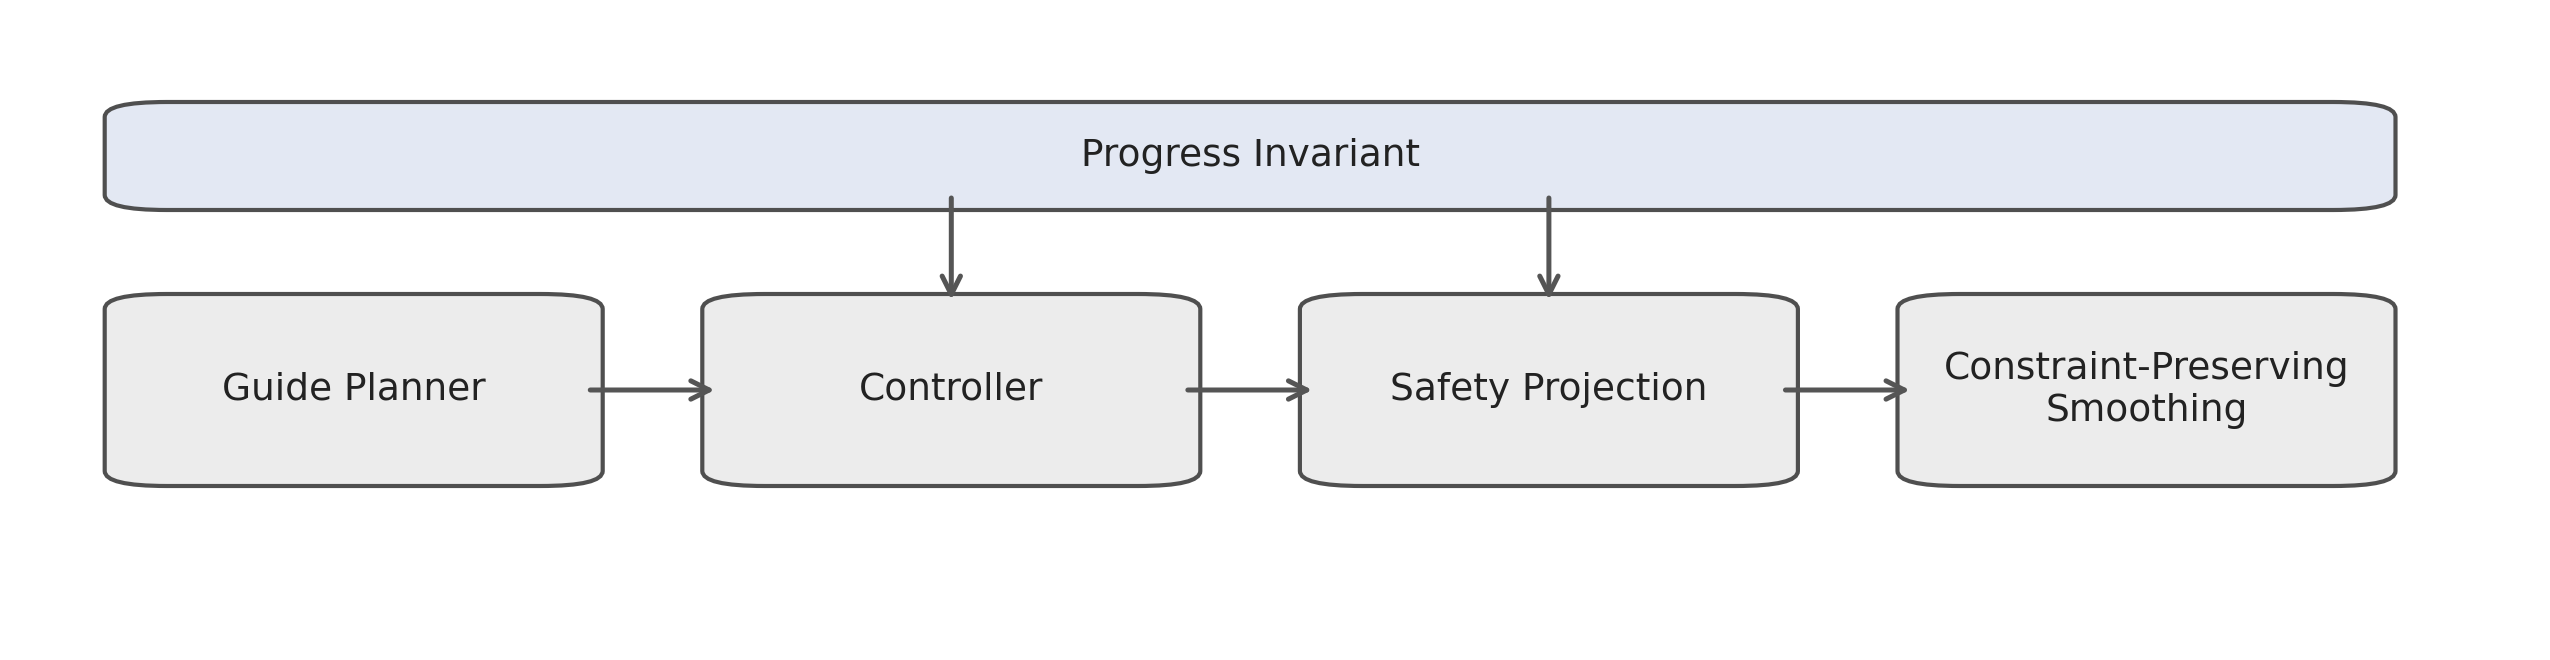
\includegraphics[width=0.85\linewidth]{../figures/pipeline.png}
  \caption{The runtime execution stack. A guide planner proposes waypoints;
  a controller turns the current target into a nominal command; a safety
  projection and smoothing layer shapes the executed command; the
  progress-regression safeguard monitors and, when necessary, corrects the
  \emph{realized} (post-projection) state at two points in the loop -- once
  on the nominal command and once after environment effects are applied.
  All quantities reported in this paper are measured on the realized state
  after this full stack, not on an intermediate command.}
  \label{fig:pipeline}
\end{figure*}

Figure~\ref{fig:pipeline} shows the runtime stack. We describe each stage
and are explicit about what each mechanism does and does not do, since
several of the results in Section~\ref{sec:results} depend on these
details.

\subsection{Guide Planner and Controller}
The guide planner exposes a sequence of static waypoints toward the goal,
computed once per scenario. The controller advances through these
waypoints and computes a nominal heading and speed toward the current
target, modulated by short-range interaction terms (weak suppression,
top-$k$ human filtering, multi-human aggregation, and short-term
interaction memory) that are individually toggleable in the ablation
configuration described in Section~\ref{sec:setup}.

\subsection{Safety Projection}
The nominal command is passed through a safety-projection layer that
enforces a minimum clearance \(d_{\text{safe}}\) (0.5\,m in all reported
scenarios) from humans and static obstacles. When the nominal step would
violate this clearance, the layer performs a bounded binary search over
candidate positions and converges to the closest point on the boundary of
the admissible region -- that is, it targets \emph{exactly}
\(d_{\text{safe}}\), not the largest available clearance. A final
hard-rollback guard prevents the executed step from crossing the
clearance threshold once the robot is already in a safe configuration.
This is a deliberate design choice (minimize deviation from the nominal
command subject to a safety constraint) and it has a direct consequence
for how the clearance and collision metrics in Section~\ref{sec:results}
should be read: because the executed state is actively projected to sit at
the safety boundary whenever the nominal command would violate it, the
minimum-clearance statistic is expected to concentrate tightly around
\(d_{\text{safe}}\) for \emph{every} controller configuration that includes
this layer, independent of any other component. We treat this as a
verification that the projection layer behaves as specified, not as an
experimental finding that discriminates between conditions.

\subsection{Progress-Regression Safeguard}
\label{sec:safeguard}
Separately from the safety projection, the controller tracks a scalar
guide-progress value \(s(k)\) -- the robot's arc-length position along the
guide path at step \(k\) -- and maintains its running maximum
\(s_{\max}(k) = \max_{j \le k} s(j)\). When the safeguard is enabled and a
candidate next state would produce \(s(k+1) < s_{\max}(k) - \varepsilon\)
for tolerance \(\varepsilon = 10^{-4}\) (the implementation's
\texttt{guide\_progress\_regression\_tolerance}), the safeguard intervenes.
The intervention is deliberately simple: it first attempts to freeze in
place (cancel the candidate step and zero the commanded velocity); a
second check applied after environment effects are integrated tries, in
order, a pre-interaction baseline position and then a full rollback to the
previous state with velocity zeroed. If neither candidate restores
\(s(k+1) \ge s_{\max}(k) - \varepsilon\) while respecting the safety
distance, the safeguard yields and the (possibly regressing) state is
executed. We emphasize that this is a bounded freeze/rollback mechanism
over at most two fallback candidates, not a replanner and not a search
procedure -- it cannot route the robot around an obstruction that the
guide planner did not already anticipate. Critically, $\varepsilon =
10^{-4}$ is an \emph{accepted-slack} threshold, not a target: the
mechanism only guarantees the executed state stays within $\varepsilon$ of
the frontier, and does not attempt to close a residual gap smaller than
$\varepsilon$ once inside it. This matters for Section~\ref{sec:results}:
our post-hoc regression-event metric (Section~\ref{sec:setup}) uses a
tighter tolerance than $\varepsilon$, so time spent by a
correctly-functioning safeguard sitting inside its own accepted slack band
can still be counted as regression by that metric.

Gated by the same flag, the controller also runs a third, independent
mechanism that we did not initially document as part of the safeguard but
that a targeted trace-level investigation (Section~\ref{sec:corridor-trap-diagnosis})
showed to be the dominant contributor to both the reported safeguard
activation counts and the safeguard's time-to-goal cost: a stall detector
that flags \emph{false progress}, \emph{stagnation}, or
\emph{progress-regressing} behavior from a sliding window of raw
Euclidean distance-to-goal (not guide-path arc length), and, when
triggered, commits the robot to a fixed lateral escape direction for a
minimum of $\max(28, 6, 12) = 28$ steps (\texttt{escape\_commit\_steps},
phase3.py:2735) before re-evaluating. This stall detector is a
goal-distance heuristic, not a check on $s(k)$ directly, and is logically
separate from the frontier freeze/rollback described above even though
both are toggled by the same ablation flag.

\subsection{Determinism and Logging}
\label{sec:repro}
All stochastic elements (per-human heading noise, crowd sampling) are
drawn from \texttt{numpy} generators seeded deterministically from the
trial seed. Every timestep of every trial is logged to a per-trial CSV
containing the realized robot state, guide progress, frontier value,
behavior state, and interaction diagnostics. \texttt{evaluation/}
\texttt{paper\_validation.py} reads these logs and regenerates every table
and figure in this paper with no additional inputs. We re-executed this
script from a clean Python environment on an unmodified checkout of the
released code and confirmed that every numeric field in every regenerated
CSV and \LaTeX{} table is identical to the committed values to full
floating-point precision; the only observed difference across the entire
regenerated output tree was an absolute filesystem path recorded for
provenance, which changes if the repository is checked out under a
different directory name.

\section{Experimental Setup}
\label{sec:setup}

\subsection{Scenarios}
We evaluate six scenarios. Four are \emph{controlled} scenarios with 50
seeds each: \textbf{Corridor Trap} (a narrow multi-obstacle corridor with
three slowly-shuffling humans near the choke point), \textbf{Crossing
Humans} (two crossing pedestrian streams), \textbf{Random Crowd} (eight
randomly sampled crossing/diagonal pedestrians per trial), and
\textbf{Structured Crowd} (five scripted crossing groups plus five
randomly sampled diagonal pedestrians, 10 humans total in expectation).
One is a \emph{stress} scenario, \textbf{Stress Crowd} (50 seeds, a dense
adversarial mix of head-on and crossing groups in a constrained corridor),
included specifically to characterize failure behavior under crowd
pressure that the controller is not expected to solve. One is a
\emph{diagnostic} scenario, \textbf{Permanent Blocking} (10 seeds, no
humans, a single solid obstacle spanning the entire width of the
workspace between start and goal, making the goal geometrically
unreachable by construction). Permanent Blocking is included to check
that the system fails safely -- without collision -- when the guide
planner's implicit feasibility assumption is violated, not to test
whether it can be solved.

\subsection{Controller Configurations}
We compare three configurations, defined as flag settings over seven
independently toggleable components (weak suppression, interaction
memory, top-$k$ filtering, multi-human aggregation, guide planner,
failed-branch memory, and the progress-regression safeguard):

\begin{itemize}
  \item \textbf{Proposed}: all seven components enabled.
  \item \textbf{No-invariant}: identical to Proposed with exactly one flag
  changed -- the progress-regression safeguard (Section~\ref{sec:safeguard})
  is disabled. This is the configuration we use to isolate the safeguard's
  effect, and it differs from Proposed in this one respect only.
  \item \textbf{Reactive baseline}: \emph{all seven} components disabled
  simultaneously, including the guide planner itself. With the guide
  planner disabled the controller has no waypoints and steers directly
  toward the raw goal position. We report this configuration because it
  is already part of the released evaluation suite, but we caution against
  reading it as an ablation of the safeguard specifically: a difference
  between Proposed and Reactive baseline is consistent with the safeguard
  mattering, with the guide planner mattering, with any of the other five
  disabled components mattering, or with some combination, and our data
  cannot distinguish among these explanations. We discuss this confound
  further in Section~\ref{sec:discussion}.
\end{itemize}

\subsection{Metrics}
We report success rate (goal reached within the step budget), a collision
proxy (minimum realized clearance falling below \(d_{\text{safe}} -
10^{-4}\)\,m), time-to-goal for successful trials, minimum realized
clearance, maximum wait and stagnation time, the safeguard's own
activation count (\emph{invariant recovery count}), and \emph{regression
events} -- the number of contiguous episodes in which realized progress
\(s(k)\) falls below the frontier \(s_{\max}(k)\) by more than
\(10^{-6}\), computed identically from the logged trajectory regardless of
which controller produced it. We deliberately use a tolerance
($10^{-6}$) two orders of magnitude tighter than the safeguard's own
accepted slack $\varepsilon = 10^{-4}$ (Section~\ref{sec:safeguard}): this
metric is meant to detect any departure from strict non-regression, not
just departures the safeguard itself considers a violation. One
consequence of this deliberate mismatch is explained in
Section~\ref{sec:corridor-trap-diagnosis}. Because regression events are
computed post-hoc from the realized trajectory using the same procedure
for every configuration, this metric is not subject to the projection
circularity described in Section~\ref{sec:safeguard} and is the metric we
rely on most heavily in Section~\ref{sec:results} to characterize the
safeguard's effect.

\section{Results}
\label{sec:results}

\subsection{Controlled Scenarios}
Table~\ref{tab:main} reports the four controlled scenarios under the
Proposed configuration. All four reach 100\% success with no recorded
collisions. Table~\ref{tab:distributions} reports the corresponding
distributions, including the safeguard's own activation count, which
varies by two orders of magnitude across scenarios (median 0 in Crossing
Humans, median 217 in Corridor Trap).

\begin{table}[t]
\centering
\scriptsize
\setlength{\tabcolsep}{2pt}
\resizebox{\linewidth}{!}{%
\begin{tabular}{@{}lccccc@{}}
\toprule
Scenario & Success & Collision & $T_{\mathrm{goal}}$ [s] & Min. clr. [m] & Unresolved recoveries \\
\midrule
Corridor Trap & 100.0\% & 0.0\% & $40.48\pm10.14$ & $0.500000\pm0.000000$ & $0.00\pm0.00$ \\
Crossing Humans & 100.0\% & 0.0\% & $9.20\pm1.28$ & $0.501\pm0.002$ & $0.00\pm0.00$ \\
Random Crowd & 100.0\% & 0.0\% & $22.80\pm6.03$ & $0.500000\pm0.000000$ & $0.00\pm0.00$ \\
Structured Crowd & 100.0\% & 0.0\% & $18.03\pm4.82$ & $0.500001\pm0.000001$ & $0.00\pm0.00$ \\
\bottomrule
\end{tabular}
}
\caption{Controlled-scenario metrics generated directly from logged run summaries. Mean and standard deviation are reported over 50 seeds per scenario.}
\label{tab:main}
\end{table}

\begin{table}[t]
\centering
\scriptsize
\setlength{\tabcolsep}{2pt}
\resizebox{\linewidth}{!}{%
\begin{tabular}{@{}lcccc@{}}
\toprule
Scenario & $T_{\mathrm{goal}}$ p50 [p25,p75] & Min. clr. p50 [p25,p75] & Max wait [s] p50 [p25,p75] & Inv. rec. p50 [p25,p75] \\
\midrule
Corridor Trap & $41.05\,[32.00,46.73]$ & $0.500000\,[0.500000,0.500000]$ & $6.30\,[3.73,7.12]$ & $217\,[136,282]$ \\
Crossing Humans & $8.75\,[8.10,9.87]$ & $0.500\,[0.500,0.500]$ & $0.85\,[0.70,1.05]$ & $0\,[0,1]$ \\
Random Crowd & $22.85\,[18.15,25.93]$ & $0.500000\,[0.500000,0.500000]$ & $1.70\,[1.00,2.45]$ & $23\,[12,40]$ \\
Structured Crowd & $18.40\,[15.12,20.83]$ & $0.500000\,[0.500000,0.500000]$ & $1.25\,[0.90,1.88]$ & $12\,[5,21]$ \\
\bottomrule
\end{tabular}
}
\caption{Distribution-aware summary from logged runs. Entries report median with interquartile range; invariant-recovery counts expose how often runtime rollback and correction were activated.}
\label{tab:distributions}
\end{table}


\subsection{Isolated Safeguard Ablation}
\label{sec:isolated-ablation}
Table~\ref{tab:noinvariant} reports the No-invariant configuration on the
same scenarios plus Stress Crowd, and, following an update to the
evaluation suite described below, Permanent Blocking. Comparing this table
to Table~\ref{tab:main}, success and failure rates are identical
scenario-for-scenario between Proposed and No-invariant. We verified this
at the seed level, not only in aggregate: across all 250 paired trials in
the five stochastic scenarios where both configurations were run (Corridor
Trap, Crossing Humans, Random Crowd, Structured Crowd, Stress Crowd),
\emph{zero trials} changed outcome between the two configurations -- no
seed exists where the safeguard converts a failure into a success or a
success into a failure.

Zero observed flips is not the same as zero statistical power to detect a
flip, so we bound the latter directly. Treating each scenario's 50 paired
trials (and the pooled 250) as independent Bernoulli trials for
"outcome changed," the exact Clopper--Pearson one-sided 95\% upper
confidence bound for a true flip probability given zero observed events
in $n$ trials is $1 - 0.05^{1/n}$. This gives an upper bound of
5.8\% (roughly 1 in 17) per individual scenario at $n=50$, and 1.2\%
(roughly 1 in 84) pooled across the five stochastic scenarios at
$n=250$. In other words, had the safeguard converted outcomes at a true
per-trial rate above roughly 1 in 17 within any single scenario, or above
roughly 1 in 84 pooled, we would have expected to observe at least one
flip in this sample; we observed none. This does not certify the absence
of arbitrarily rare effects, but it rules out a moderate-or-larger
effect on success/failure outcomes with a stated confidence level, rather
than resting the null claim on sample size alone.

\begin{table}[t]
\centering
\scriptsize
\setlength{\tabcolsep}{2pt}
\resizebox{\linewidth}{!}{%
\begin{tabular}{@{}lcccc@{}}
\toprule
Scenario & Failure & Regression events p50 [p25,p75] & Max wait [s] p50 [p25,p75] & Dominant mode \\
\midrule
Corridor Trap & 0.0\% & $0\,[0,0]$ & $1.60\,[1.52,1.70]$ & none \\
Crossing Humans & 0.0\% & $0\,[0,0]$ & $0.85\,[0.70,1.40]$ & none \\
Random Crowd & 0.0\% & $1\,[0,2]$ & $2.40\,[2.00,2.88]$ & none \\
Structured Crowd & 0.0\% & $0\,[0,0]$ & $1.70\,[1.40,2.30]$ & none \\
Stress Crowd* & 100.0\% & $6\,[5,8]$ & $9.70\,[8.48,11.78]$ & deadlock \\
\bottomrule
\end{tabular}
}
\caption{Invariant-off ablation generated from logged runs. Regression events count episodes in which executed progress falls below the previously attained frontier.}
\label{tab:noinvariant}
\end{table}


The safeguard's effect on the regression-event and time-to-goal metrics it
targets is inconsistent across scenarios and, in one case, moves in the
direction opposite to its intent. Table~\ref{tab:ablation-detail}
summarizes the paired totals computed directly from the per-trial logs;
unlike in an earlier version of this evaluation suite, this table is now
part of the automatically regenerated table set
(\texttt{evaluation/paper\_validation.py}), so it is no longer an
exception to the reproducibility claim of Section~\ref{sec:repro}.

\begin{table}[h]
\centering
\scriptsize
\caption{Paired totals per scenario/configuration, Proposed (safeguard on) vs.\ No-invariant (safeguard off), over the trial count reported in Table~\ref{tab:main}/\ref{tab:noinvariant}. Regression events and time-to-goal are computed identically for both configurations.}
\label{tab:ablation-detail}
\begin{tabular}{@{}lcccc@{}}
\toprule
Scenario & \multicolumn{2}{c}{Regr.\ events (sum)} & \multicolumn{2}{c}{Mean $T_{\text{goal}}$ [s]} \\
 & On & Off & On & Off \\
\midrule
Corridor Trap & 60 & 1 & 40.48 & 20.24 \\
Crossing Humans & 1 & 0 & 9.20 & 9.19 \\
Random Crowd & 17 & 52 & 22.80 & 22.66 \\
Structured Crowd & 7 & 5 & 18.03 & 19.49 \\
Stress Crowd* & 166 & 322 & n/a (0.0\%) & n/a (0.0\%) \\
\bottomrule
\end{tabular}
\end{table}


In Corridor Trap the safeguard is associated with \emph{sixty times more}
regression events than disabling it (60 vs.\ 1 over 50 trials) and
approximately doubles mean time-to-goal (40.48\,s vs.\ 20.24\,s), while
success remains 100\% in both configurations. The same pattern also
appears in a metric neither this table nor Table~\ref{tab:main} reports
directly: median max-wait time for Corridor Trap is 6.30\,s under Proposed
(Table~\ref{tab:distributions}) but only 1.60\,s under No-invariant
(Table~\ref{tab:noinvariant}) -- a $4\times$ swing on the same 50 seeds,
larger in relative terms than the time-to-goal doubling, and driven by the
same root cause (Section~\ref{sec:corridor-trap-diagnosis}). In Random
Crowd the safeguard is associated with fewer regression events, in the
direction its design intends; Stress Crowd shows the same direction (166
vs.\ 322) but we do not treat this as supporting evidence, since both
configurations fail 100\% of trials there and a regression-event
difference between two arms that both fail is not cleanly interpretable
as the safeguard \emph{working} -- it may simply be two different flavors
of failing. In Structured Crowd and Crossing Humans the effect is small in
both directions.

We initially reported this Corridor Trap result without a confirmed
mechanistic explanation. A subsequent trace-level investigation --
instrumenting one representative Proposed trial (seed 0) with per-step
logging of which recovery branch fired, gated behind a debug flag removed
before this table was finalized -- identified two distinct, confirmed
causes, detailed in Section~\ref{sec:discussion}.
\label{sec:corridor-trap-diagnosis}
Figures~\ref{fig:recovery} and~\ref{fig:time} corroborate the pattern
visually: Corridor Trap is the clear outlier in both safeguard activation
count and time-to-goal spread among the controlled scenarios.

We initially had no ablation data for Permanent Blocking; we closed this
gap by enabling the existing No-invariant and Reactive-baseline dispatch
for that scenario and re-running the pipeline (10 newly generated seeds).
Since Permanent Blocking contains no humans, all 10 seeds under a given
configuration are identical -- a confirmed single-configuration effect,
not independent statistical variation (Table~\ref{tab:noinvariant}'s
$[3,3]$ interquartile range reflects this). The effect is real and
different in character from the crowd scenarios: with the safeguard
enabled, the robot has zero regression events but persists for 73.3\,s
and 762 activations before exhausting its step budget; with it disabled
(No-invariant and Reactive baseline are numerically identical here, since
neither the guide planner nor any other disabled component has anything
to act on without humans), 3 regression events occur but the controller
recognizes stagnation and gives up after 2.2\,s. Success and collision
are 0\%/0\% in both cases regardless. The safeguard's only confirmed
effect here is to trade a fast, regressing failure for a slow,
non-regressing one -- it holds the line against regression at the cost of
persisting far longer in a provably infeasible situation.

\begin{figure}[t]
  \centering
  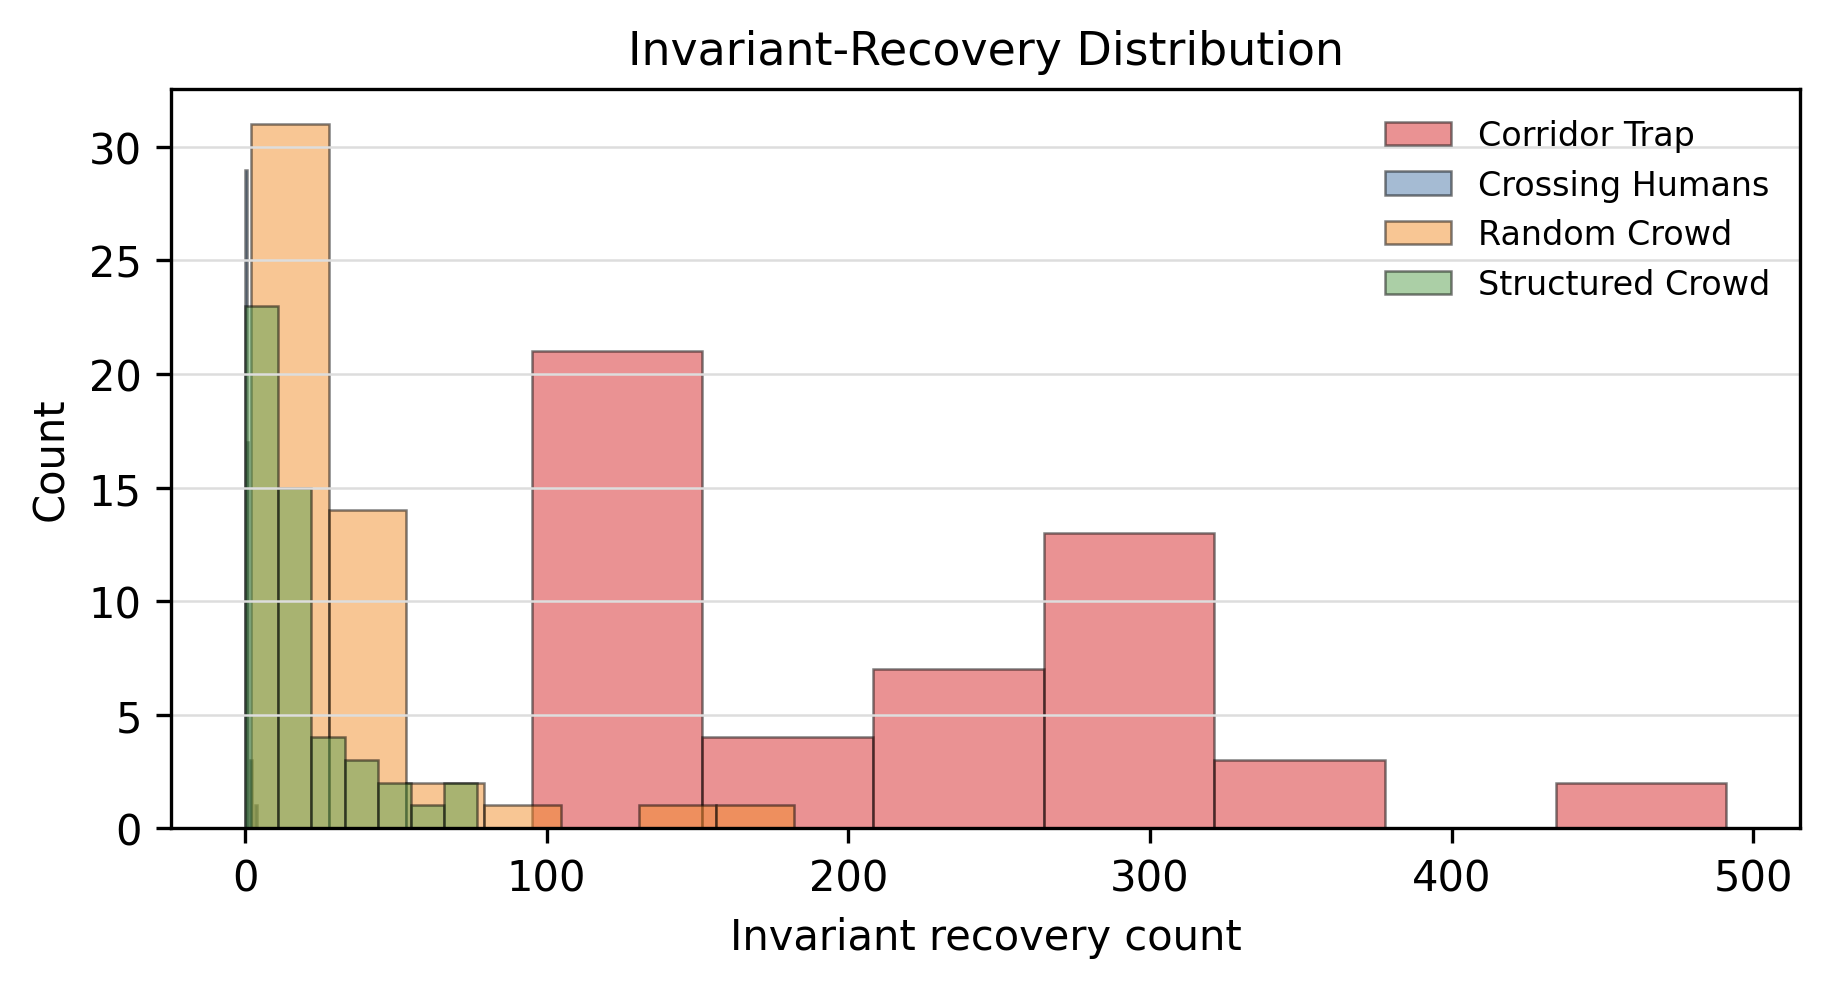
\includegraphics[width=0.85\linewidth]{../figures/recovery_hist.png}
  \caption{Distribution of safeguard activation count (invariant recovery
  count) per trial, Proposed configuration, controlled scenarios. Corridor
  Trap is a clear outlier, consistent with Table~\ref{tab:ablation-detail}.}
  \label{fig:recovery}
\end{figure}

\begin{figure}[t]
  \centering
  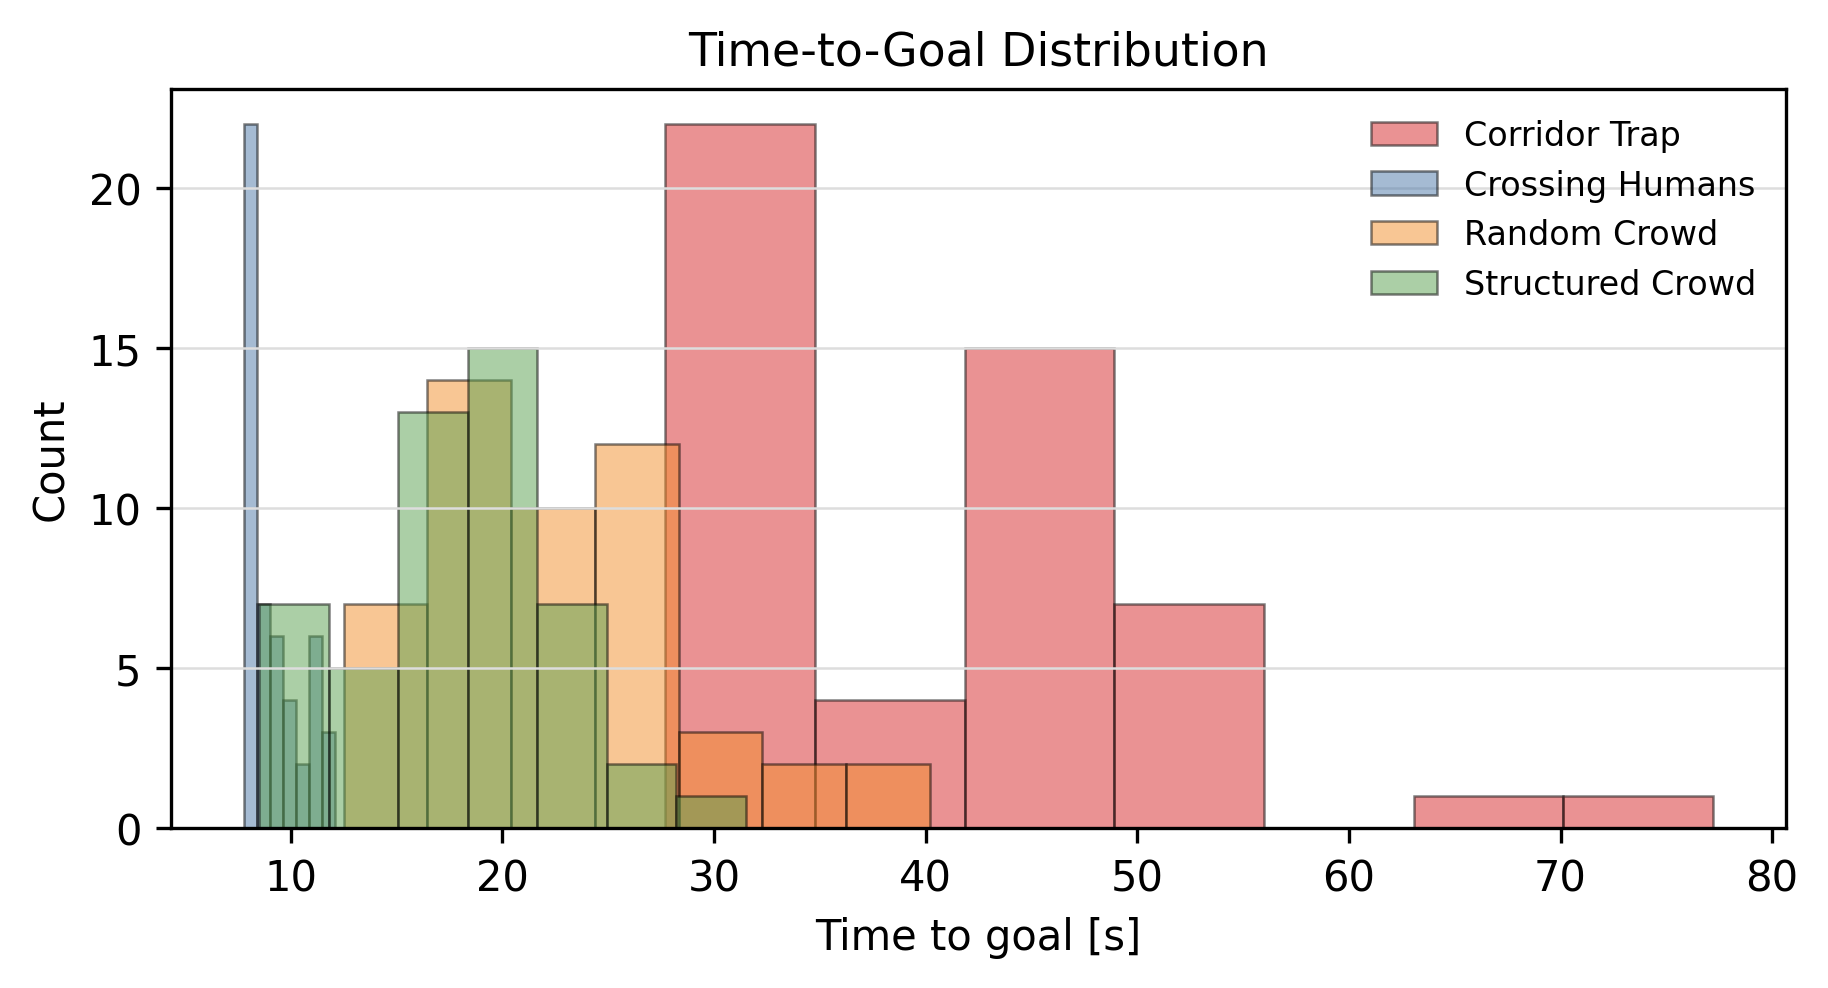
\includegraphics[width=0.85\linewidth]{../figures/time_hist.png}
  \caption{Distribution of time-to-goal per trial, Proposed configuration,
  controlled scenarios. Corridor Trap shows a long right tail (up to
  77\,s) not present in the other three scenarios.}
  \label{fig:time}
\end{figure}

\subsection{Reactive Baseline Comparison}
Table~\ref{tab:baseline} reports the Reactive baseline configuration.
Proposed outperforms it by a wide margin in Corridor Trap (100\% vs.\ 0\%
success) and Random Crowd (100\% vs.\ 2\% success), and is comparable in
Crossing Humans (100\% vs.\ 100\%). As stated in
Section~\ref{sec:setup}, this configuration disables the guide planner in
addition to the safeguard and five other components; with the guide
planner disabled the controller steers directly at the raw goal with no
route around obstacles, which alone is sufficient to explain failure in
an obstacle-obstructed scenario such as Corridor Trap. We report this
comparison for completeness because it is part of the released evaluation
suite, but given the results in Table~\ref{tab:ablation-detail} we do
\emph{not} interpret it as evidence for the safeguard: the isolated,
single-variable ablation directly above is the correct comparison for
that question, and it shows no effect on outcome.

\begin{table}[t]
\centering
\scriptsize
\setlength{\tabcolsep}{2pt}
\resizebox{\linewidth}{!}{%
\begin{tabular}{@{}llcccc@{}}
\toprule
Scenario & Controller & Success & Collision & $T_{\mathrm{goal}}$ [s] & Min. clr. [m] \\
\midrule
Corridor Trap & Proposed & 100.0\% & 0.0\% & $40.48\pm10.14$ & $0.500000\pm0.000000$ \\
Corridor Trap & Reactive baseline & 0.0\% & 0.0\% & -- & $0.500000\pm0.000000$ \\
Crossing Humans & Proposed & 100.0\% & 0.0\% & $9.20\pm1.28$ & $0.501\pm0.002$ \\
Crossing Humans & Reactive baseline & 100.0\% & 0.0\% & $9.08\pm1.34$ & $0.501\pm0.002$ \\
Random Crowd & Proposed & 100.0\% & 0.0\% & $22.80\pm6.03$ & $0.500000\pm0.000000$ \\
Random Crowd & Reactive baseline & 2.0\% & 0.0\% & $27.00$ (n=1) & $0.500000$ (n=1) \\
\bottomrule
\end{tabular}
}
\caption{Comparison against a reactive baseline that retains only runtime safety projection: the guide planner, weak suppression, interaction memory, top-$k$ filtering, multi-human aggregation, failed-branch memory, and the progress-regression safeguard are all disabled simultaneously (7 flags). This is not a single-variable ablation of the safeguard; see Table~\ref{tab:noinvariant} for that comparison. Time-to-goal is reported over successful runs only.}
\label{tab:baseline}
\end{table}


\subsection{Failure Behavior}
Table~\ref{tab:failures} reports diagnostics for the two scenarios in
which the controller does not reach the goal. Stress Crowd fails on 100\%
of trials with zero collisions and a deadlock-dominant failure mode.
Figure~\ref{fig:failure} shows the Stress Crowd trial (Proposed
configuration) selected by our evaluation script as the single worst-case
failure by maximum wait time among that scenario's 50 seeds -- it is the
most extreme observed case, not a typical or averaged one. The robot is
held at the safety boundary of an obstruction rather than crossing it or
colliding with it.

Permanent Blocking fails on 100\% of trials (as expected, since the goal
is geometrically unreachable by construction) with zero collisions and a
maximum wait time of 76.1\,s under the Proposed configuration. Unlike
Stress Crowd, this scenario contains no humans, so all 10 seeds under a
given configuration produce an identical trajectory
(Section~\ref{sec:isolated-ablation}) -- there is no representative or
worst-case seed to select here, every seed is the same outcome.
Table~\ref{tab:failures} reports only the Proposed configuration for both
scenarios; the corresponding No-invariant and Reactive-baseline ablation
for Permanent Blocking is reported and discussed in
Section~\ref{sec:isolated-ablation} and Table~\ref{tab:noinvariant} --
disabling the safeguard does not change the 0\% success or 0\% collision
rate there, but reduces the reported wait time in this table from
76.1\,s to 10.2\,s, consistent with the safeguard prolonging a failure it
cannot ultimately prevent.

\begin{table}[t]
\centering
\scriptsize
\setlength{\tabcolsep}{2pt}
\resizebox{\linewidth}{!}{%
\begin{tabular}{@{}lccccc@{}}
\toprule
Scenario & Failure & Collision & Unresolved recoveries & Max wait p75 [s] & Dominant mode \\
\midrule
Corridor Trap & 0.0\% & 0.0\% & $0.00\pm0.00$ & 7.1 & none \\
Crossing Humans & 0.0\% & 0.0\% & $0.00\pm0.00$ & 1.1 & none \\
Random Crowd & 0.0\% & 0.0\% & $0.00\pm0.00$ & 2.5 & none \\
Structured Crowd & 0.0\% & 0.0\% & $0.00\pm0.00$ & 1.9 & none \\
Stress Crowd* & 100.0\% & 0.0\% & $0.22\pm0.41$ & 11.1 & deadlock \\
Permanent Blocking** & 100.0\% & 0.0\% & $0.00\pm0.00$ & 76.1 & deadlock \\
\bottomrule
\end{tabular}
}
\caption{Failure-oriented diagnostics derived from logged runs. The starred stress row is a logged adversarial crowd suite used to expose safe failure; the double-starred permanent-blocking row is an out-of-regime diagnostic used to illustrate behavior when admissible-dynamics assumptions are violated.}
\label{tab:failures}
\end{table}


\begin{figure}[t]
  \centering
  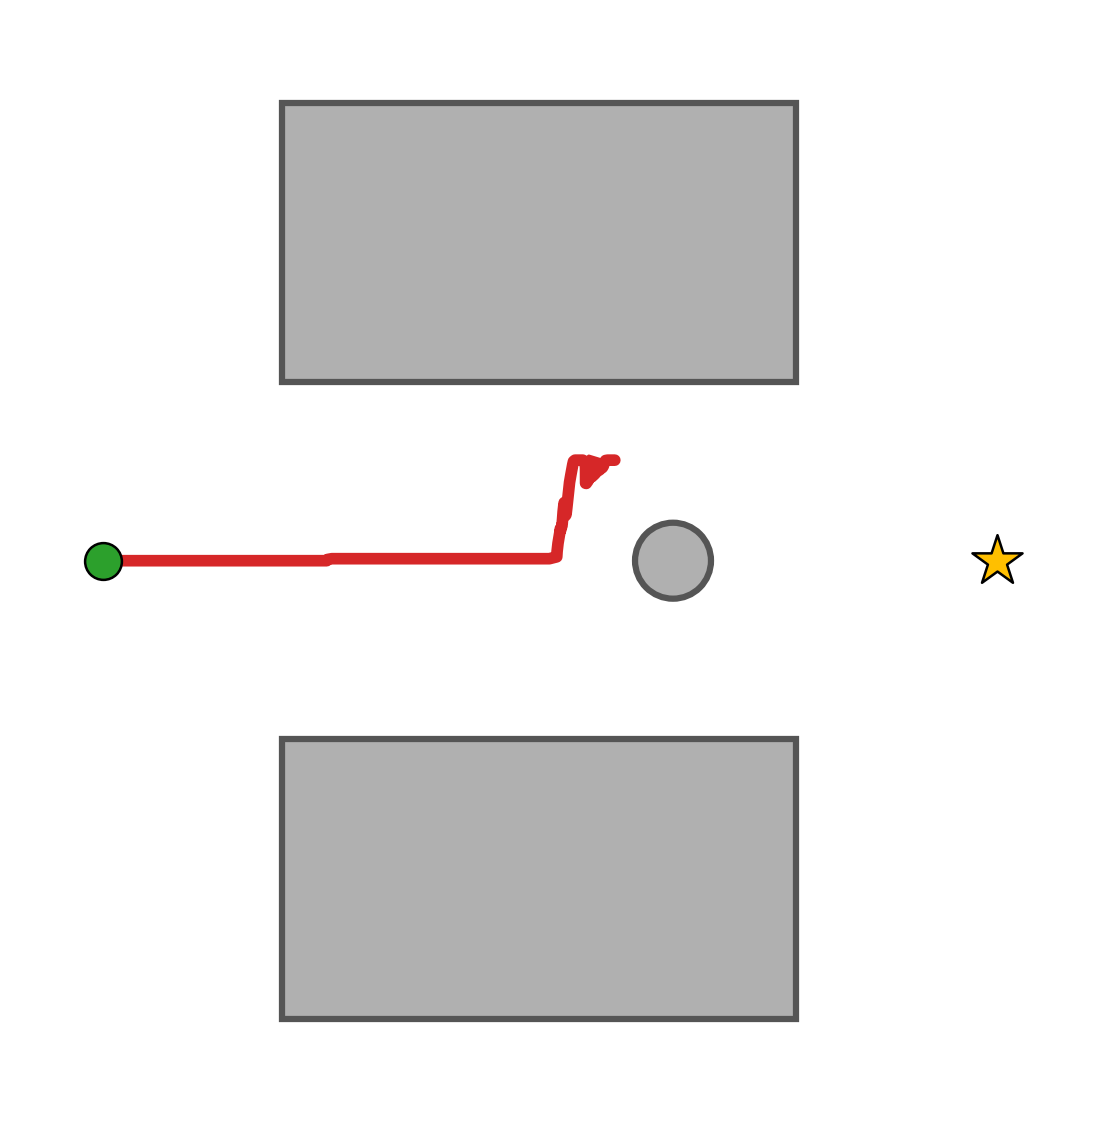
\includegraphics[width=0.8\linewidth]{../figures/failure_case.png}
  \caption{The Stress Crowd trial (Proposed configuration) with the
  largest recorded wait time among its 50 seeds: the robot is held at the
  safety boundary of an obstruction rather than crossing it or colliding.}
  \label{fig:failure}
\end{figure}

\section{Discussion}
\label{sec:discussion}

\textbf{The safeguard does not measurably improve task success in this
scenario suite.} The isolated ablation in
Table~\ref{tab:noinvariant}/Table~\ref{tab:ablation-detail} is, by
construction, the correct experiment for this question, and it returns a
null result at the seed level across 250 trials. We do not think this
result should be explained away: it is the direct output of a
correctly-isolated single-variable ablation, run at a large enough number
of seeds (50 per scenario) that a consistent effect of moderate size
would be expected to appear if one existed.

\textbf{The safeguard's effect on its own target metric is
scenario-dependent, and in one case adverse -- and we now have a confirmed,
not merely hypothesized, explanation for Corridor Trap.} We instrumented
one representative Proposed trial (seed 0) with per-step branch-level
logging (gated behind a debug flag, removed after use; no committed
behavior was changed) and traced every activation of the freeze/rollback
mechanism and the goal-distance stall detector introduced in
Section~\ref{sec:safeguard}. Two distinct, confirmed effects combine:

\emph{(i) A tolerance-mismatch metric artifact.} The regression-event
count is inflated by the deliberate mismatch between the safeguard's
accepted slack ($\varepsilon = 10^{-4}$) and the metric's tolerance
($10^{-6}$, Section~\ref{sec:setup}). In the traced trial, the
frontier-vs-progress gap jumps to exactly $5.456\times10^{-5}$ at one step
and then holds at that constant value for 68 further consecutive steps
while the robot's position keeps changing -- comfortably inside the
safeguard's accepted $10^{-4}$ band (so the enforcement mechanism
correctly does not intervene further) but 54$\times$ larger than the
metric's $10^{-6}$ threshold (so it is counted as an ongoing regression
episode for the entire 6.8 s it persists). This single episode is the
trial's one logged regression event, spanning the 69 regression-steps
recorded for it. Without the safeguard, nothing actively holds the
trajectory near this boundary, so such persistent small gaps are rare
(1 event across 50 Corridor Trap seeds, vs.\ 60 with the safeguard on).

\emph{(ii) An inherent design cost in the stall detector, not the
frontier check.} The same trace shows the freeze/rollback mechanism
(Stage 1/2) firing only 30 times in this trial, always resolved by the
baseline-position candidate, never needing full rollback and never
failing -- it is not thrashing. The dominant activity, and the dominant
driver of both the time-to-goal and max-wait cost documented above, is
the separate goal-distance stall detector (Section~\ref{sec:safeguard}):
288 of the trial's 463 steps (62\%) show it active, spanning 11 separate
committed 28-step escape holds. Corridor Trap places three near-stationary
humans (preferred speed 0.05) directly in the only feasible gap of the
robot's detour path; passing them requires sustained lateral movement that
does not reduce raw goal distance, which the detector repeatedly
misreads as stalling, re-triggering a fresh 28-step commitment each time
the previous one expires while the robot is still working past the
cluster. This is a genuine design limitation -- a goal-distance-only
heuristic is a poor proxy for whether a lateral detour is legitimate --
not a coding defect: the mechanism does exactly what its logic specifies,
and net position advances monotonically across corrections (no
oscillation, no repeated visits to the same state). No other controlled
scenario places a near-stationary human cluster directly in a mandatory
single-file pinch point the way Corridor Trap does, which is consistent
with Corridor Trap being the outlier by roughly two orders of magnitude in
Figure~\ref{fig:recovery}. We verified this mechanism on one representative
trial rather than across all 50 Corridor Trap seeds; we treat it as the
confirmed proximate cause for that trial and the most likely explanation
for the aggregate pattern, not as separately verified for every seed.

\textbf{The Reactive-baseline comparison should not be read as evidence
about the safeguard.} It differs from Proposed in seven components at
once, one of which is the entire guide planner. A large success-rate gap
under this comparison is compatible with several different single-cause
explanations, and our data does not distinguish among them. We consider
the isolated No-invariant ablation the authoritative comparison for the
safeguard specifically, and we would caution any reader of the earlier
figures in this evaluation suite against treating the Reactive-baseline
numbers as if they isolated the safeguard's contribution.

\textbf{The clearance and collision metrics verify the projection layer,
not the safeguard.} As noted in Section~\ref{sec:safeguard}, the
minimum-clearance statistic is expected to concentrate near
\(d_{\text{safe}}\) for any configuration that retains the safety
projection layer, independent of the safeguard, the guide planner, or any
other component -- and Table~\ref{tab:noinvariant}'s underlying data
confirms this: minimum clearance is statistically indistinguishable
between Proposed and No-invariant. We report it because it verifies that
the projection layer is functioning as designed, and we caution against
reading the resulting 0\% collision rate as evidence specifically
attributable to the safeguard.

\section{Limitations}
\label{sec:limitations}

\begin{itemize}
  \item \textbf{No external baseline.} All comparisons in this paper are
  internal ablations of a single codebase. We do not compare against
  independent implementations of ORCA, the Social Force Model, or DWA
  despite citing them as related work; doing so is necessary before any
  claim of comparative performance against the broader
  literature~\cite{social_force,orca,dwa} can be supported.
  \item \textbf{Permanent Blocking is a single deterministic configuration,
  not a distribution.} We closed the ablation gap for this scenario
  (Section~\ref{sec:isolated-ablation}), but because it contains no humans
  every seed under a given configuration produces an identical trajectory;
  the reported comparison is a confirmed single-instance effect, not a
  statistically distributed one, and should not be read with the same
  statistical weight as the 250-trial ablation in the five stochastic
  scenarios.
  \item \textbf{Simulation fidelity.} The robot is modeled as a 2D
  kinematic point mass with velocity smoothing and no acceleration or
  actuator limits, and clearance is computed from exact, noise-free
  ground-truth positions rather than from a simulated sensor. This is a
  substantially lower-fidelity model than the dynamics of a real
  differential-drive or holonomic platform, and no hardware validation is
  reported in this paper.
  \item \textbf{The Corridor Trap diagnosis (Section~\ref{sec:discussion})
  was verified on one representative trial, not all 50 seeds.} We
  instrumented and traced a single seed rather than exhaustively confirming
  the same mechanism across every Corridor Trap trial; we treat it as the
  confirmed cause for that trial and the most likely explanation for the
  aggregate pattern, not as independently verified per seed.
\end{itemize}

\section{Conclusion}

We built a deterministic, fully log-reproducible simulation and evaluation
pipeline for a guide-planner-based social-navigation controller with a
runtime safety-projection layer, and used it to run a correctly-isolated,
single-variable ablation of an execution-level progress-regression
safeguard across 250 paired trials in five scenarios. The honest result of
that ablation is that the safeguard changes no success/failure outcome at
the seed level and has a scenario-dependent, occasionally adverse, effect
on the regression and time-to-goal metrics it targets. We consider the
deterministic execution and evaluation pipeline -- together with the
guide-planner-based controller and its safety-projection layer, all
independently re-verified to reproduce bit-identically from logged data --
to be this paper's defensible contribution, and we report the
safeguard's ablation as a negative/mixed result rather than reframe or
omit it. We release the full per-seed dataset, code, and evaluation
script so that these conclusions, and any future ones built on this
codebase, can be checked directly against logged execution traces rather
than taken on faith.

{\small
\bibliographystyle{ieeetr}
\bibliography{references}
}

\end{document}
